\documentclass{article}
\title{The Ant Colony Optimisation for the Travelling Salesman Problem}
\author{Dylan Galea}

\usepackage{cite}
\usepackage{amsmath}
\usepackage{amsthm}
\usepackage{amssymb}
\usepackage{physics}
\usepackage{tikz}
\usepackage{slashbox}
\usetikzlibrary{arrows.meta,automata,positioning}

\newtheorem{definition}{Definition}[subsection]
\newtheorem{theorem}[definition]{Theorem}
\newtheorem{lemma}[definition]{Lemma}
\newtheorem*{remark}{Remark}
\newtheorem{example}[definition]{Example}

\begin{document}
\maketitle
\newpage
\tableofcontents
\newpage
\section{Introduction}
Before defining the Travelling Salesman Problem and proving properties about it, a number of graph theoretic concepts that will be used throughout, must first be defined. Therefore, what follows is a sub-section that introduces a number of graph theoretic concepts which are required for the Travelling Salesman Problem.
\subsection{Some Graph Theory}
Graph theory is the study of a structure called a graph. A graph can be defined formally as shown in definition \ref{Graph} below.
\begin{definition}
\label{Graph}
A graph G is a pair (V,E) were V is any non empty finite set called the set of vertices of G, and E $\subseteq$ \{$\{u,v\}$ $:$ $\forall$ u,v $\in$ V and u $\neq$ v\} is called the set of edges of G {\normalfont{\cite{black_tanenbaum_2017}}}. A graph G defined by the pair (V,E) is denoted by G(V,E) or G.
\end{definition}
A graph defined using definition \ref{Graph} is called an undirected graph. There is also the concept of a directed graph were $\mathit{E \subseteq \{(u,v) : \forall u,v \in V, u \neq v\}}$ \cite{black_tanenbaum_2017}. However, in this thesis it can be assumed that any graph that will be considered is undirected unless otherwise stated. It can also be assumed that there are no edges between same vertices unless otherwise stated. It must also be noted that by this definition, there cannot be multiple edges joining any 2 vertices. The reason is that sets do not allow repetition of elements. Thus, each element in the edge set is unique. The discussion will now proceed by introducing more graph theoretic terminology, with examples that illustrate these terminologies.\\
\\When two vertices are joined by an edge, they are said to be adjacent. This is defined formally in definition \ref{adjacent} below.
\begin{definition}
\label{adjacent}
Given a graph G(V,E), $\forall$ u,v $\in$ V, u and v are said to be adjacent if \{$u,v\}$ $\in$ E. Also, if u and v are adjacent, then u and v are said to be end vertices of the edge \{$u,v\}$. \normalfont{\cite{harris_hirst_mossinghoff_2008}}
\end{definition}
There is also a special name associated with the case when a vertex is an end vertex of an edge.
\begin{definition}
\label{incident}
A vertex v in a graph G is incident to an edge e in G if v is an end vertex of e. {\normalfont{\cite{harris_hirst_mossinghoff_2008}}}
\end{definition}
It is sometimes also required to know how many edges are incident to a specific vertex in a graph.
\begin{definition}
\label{degree}
The degree of a vertex v in a graph G denoted by deg(v) is, the number of edges incident with v in G. {\normalfont{\cite{harris_hirst_mossinghoff_2008}}}
\end{definition}
Any graph $\mathit{G(V,E)}$ can also be represented pictorially by drawing the vertices of $\mathit{G}$ using circles, and by drawing the edges of $\mathit{G}$ using lines between adjacent vertices. As a result, in this thesis a graph is sometimes given formally using sets or as a pictorial representation, assuming that one can be converted into another. Example \ref{Example 1} below depicts how a graph can be represented pictorially.
\begin{example}
\label{Example 1}
{\normalfont{Consider the graph}} G(V,E) {\normalfont{such that}}  V=\{$v_1, v_2, v_3, v_4\}$ {\normalfont{and}} E = \{$\{v_1, v_2\}, \{v_2,v_3\}, \{v_3,v_4\}, \{v_4,v_1\}\}$.\\{\normalfont{Then}} G {\normalfont{can be represented pictorially as :}}\\

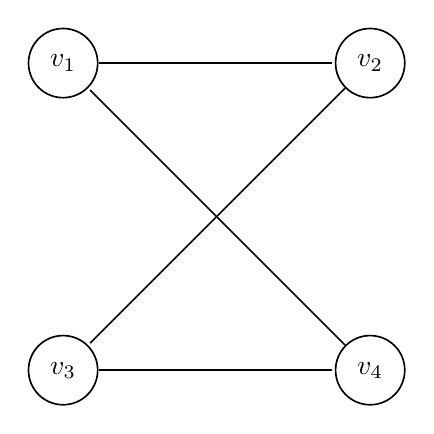
\begin{tikzpicture}[
    > = , % arrow head style
    shorten > = 1pt, % don't touch arrow head to node
    auto,
    node distance = 3cm, % distance between nodes
    semithick % line style
    ]

    \tikzset{every state}=[
    draw = black,
    thick,
    fill = black,
    minimum size = 1mm
    ]

    \node[state] (v1) {$v_1$};
    \node[state] (v2) [right=of v1] {$v_2$};
    \node[state] (v3) [below =of v1] {$v_3$};
    \node[state] (v4) [below =of v2] {$v_4$};
  
    \path[->] (v1) edge  node[]{}(v2);
    \path[->] (v2) edge  node[]{} (v3);
    \path[->] (v3) edge  node[]{}(v4);
    \path[->] (v4) edge  node[]{}(v1);
\end{tikzpicture}\\
{\normalfont{Using definition \ref{adjacent}, two adjacent vertices in }}G {\normalfont{are}} $v_1$ {\normalfont{and}} $v_2$.{\normalfont{ On the other hand, two non adjacent vertices in }}G {\normalfont{are}} $v_1$ {\normalfont{and}} $v_3.$\\ {\normalfont{By definition \ref{incident}}}, $v_1$ {\normalfont{and}} $v_2$ {\normalfont{are incident to the edge}} \{$v_1, v_2\}$.\\
{\normalfont{Using definition \ref{degree}, the degree of every vertex in}} G {\normalfont{is 2}}.
\end{example}
There are many other examples of graphs, one of them being the complete graph on $\mathit{n}$ vertices.
\begin{definition}
\label{Complete Graph}
A graph G(V,E) is said to be complete if $\forall$ v,w $\in$ V v $\neq$ w, v is adjacent to w. The complete graph on n vertices is denoted by $K_n$. \normalfont{\cite{harris_hirst_mossinghoff_2008}}
\end{definition}
Given any graph $\mathit{G(V,E)}$, one can also define graph theoretic structures that lie within $\mathit{G}$, one of them being a path.
\begin{definition}
\label{Path}
Given a graph G(V,E), a path in G joining any 2 vertices u, v $\in$ V, is a sequence of vertices u = $u_1$, $u_2$, ...,$u_n$ = v in which no vertex is repeated and, $\forall$ 0 $<$  i $<$ n, \{$u_i, u_{i+1}\}$ $\in$ E. {\normalfont{\cite{thompson}}}
\end{definition}
Definition \ref{Path} can now be used to define cycles and connectivity in a graph.
\begin{definition}
\label{connectedgraph}
A graph G(V,E) is said to be connected if $\forall$ u,v $\in$ V u $\neq$ v, u and v are joined by a path. \normalfont{\cite{harris_hirst_mossinghoff_2008}}
\end{definition}
\begin{definition}
\label{cycle}
Given a graph G(V,E), a cycle in G is a path on n $\geq$ 4 vertices, such that, the first vertex and the last vertex are equal. \normalfont{\cite{cycle}} 
\end{definition}
By definitions \ref{Path}, \ref{cycle} above, it is clear that a cycle is a special instance of a path, with the only difference being that in a cycle, the first vertex and the last vertex are equal. Another thing worth mentioning is that, according to definitions \ref{Path} and \ref{cycle}, cycles and paths are sequences of vertices and not actual graphs. However, this is not the case because they can be represented easily as graphs. For example, given the path/cycle $\mathit{u_1, u_2, ...,u_n}$ a new graph $\mathit{G(V,E)}$ can be created such that, $\mathit{V(G)= \{ u_1, u_2, ..., u_n\}}$ and $\mathit{E(G) = \{ \{u_i, u_{i+1}\} : \forall i, 0 < i < n\}}$. For example, consider the cycle v1 v2 v3 v4 v1, then the graph depicted in example \ref{Example 1}, is the graph representing this cycle. Such graphs are known as Cycle/Path graphs and are denoted by $\mathit{C_n/P_n}$ respecitvely, $\mathit{n}$ being the number of vertices in the graph. Since this construction can be done, cycles/paths will be treated as both graphs and sequences. This will later be useful when defining Hamiltonian cycles. For better understanding of definitions \ref{Complete Graph}, \ref{Path}, \ref{connectedgraph} and \ref{cycle}, example \ref{example3} is constructed.
\begin{example}
\label{example3}
{\normalfont{Consider the graph}} G(V,E) {\normalfont{below:}}\\
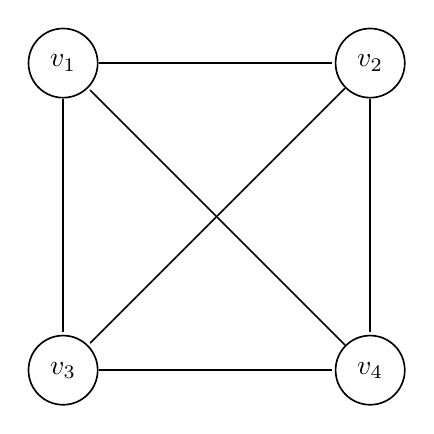
\begin{tikzpicture}[
    > = , % arrow head style
    shorten > = 1pt, % don't touch arrow head to node
    auto,
    node distance = 3cm, % distance between nodes
    semithick % line style
    ]

    \tikzset{every state}=[
    draw = black,
    thick,
    fill = black,
    minimum size = 1mm
    ]

    \node[state] (v1) {$v_1$};
    \node[state] (v2) [right=of v1] {$v_2$};
    \node[state] (v3) [below =of v1] {$v_3$};
    \node[state] (v4) [below =of v2] {$v_4$};
  
    \path[->] (v1) edge  node[]{}(v2);
    \path[->] (v1) edge  node[]{}(v3);
    \path[->] (v2) edge  node[]{} (v3);
    \path[->] (v3) edge  node[]{}(v4);
    \path[->] (v2) edge  node[]{}(v4);
    \path[->] (v4) edge  node[]{}(v1);
\end{tikzpicture}
\\
{\normalfont{Since every vertex in}} G {\normalfont{is adjacent to every other vertex, }}G {\normalfont{must be complete. Therefore}} G {\normalfont{must be}} $K_4$. {\normalfont{Since}} G {\normalfont{is complete, it must also be connected because, there is a path}} $P_2$ {\normalfont{between any 2 distinct vertices of}} G.\\
{\normalfont{Some examples of paths in}} G {\normalfont{are:}}\\
1. $v_1$ $v_2$ $v_3$ $v_4$\\
2. $v_1$ $v_4$\\
3. $v_4$ $v_3$ $v_1$\\
{\normalfont{Some examples of cycles in}} G {\normalfont{are:}}\\
1. $v_1$ $v_2$ $v_3$ $v_4$ $v_1$\\
2. $v_1$ $v_4$ $v_2$ $v_3$ $v_1$\\
3. $v_4$ $v_3$ $v_1$ $v_4$
\end{example}
Another important graph theoretic concept is that of subgraphs. 
\begin{definition}
\label{subgraph}
Given a graph G(V,E) and a graph H($V^\prime$,$E^\prime$), H is a subgraph of G if $V^\prime$ $\subseteq$ V and $E^\prime$ $\subseteq$ E.  \normalfont{\cite{harris_hirst_mossinghoff_2008}}
\end{definition}
After defining some important concepts, the next step is to extend definition \ref{Graph} to define another class of graphs called weighted graphs. It must be noted that all definitions presented so far apply also to weighted graphs.
\begin{definition}
\label{Weighted Function}
Given a graph G(V,E), a weight function is a function f : E $\mapsto$ $\real^+$ {\normalfont{\cite{harris_hirst_mossinghoff_2008}}}. The real numbers assigned to each edge are called weights.
\end{definition}
Note that in definition \ref{Weighted Function}, the weights are taken to be positive. According to \cite{harris_hirst_mossinghoff_2008}, there could be cases were negative weights would be appropiate. However, unless otherwise stated, it is to be assumed that when considering a weight function, the weights are positive.
\begin{definition}
\label{Weighted Graph}
A weighted graph is a graph G(V,E) with a weight function f {\normalfont{\cite{harris_hirst_mossinghoff_2008}}}. This is denoted by the triple G(V,E,f) or G. 
\end{definition}
According to Bondy and Murty \cite{bondy_murty_1982}, weighted graphs occur regularly in applied graph theory. For example, a railway network can be represented by a weighted graph were, the vertices are the set of towns in the railway network, and there are edges between 2 vertices in the graph if, there is a direct route from one town to another, without visiting other towns in the process. The weight function would then represent the cost of travelling directly from one town to another. In addition to that, the shortest path between 2 towns in the network may be required. It is clear that in order to try and solve such problems, the total weight of a subgraph must first be defined.
\begin{definition}
\label{weightofasubgraph}
Given a weighted graph G(V,E,f), the total weight of any subgraph  H($V^\prime$,$E^\prime$,f) of G is: $$\sum_{e \in E^\prime}^{} f(e) $$. \normalfont{\cite{bondy_murty_1982}}
\end{definition}
It is important to note that by definition \ref{subgraph}, any weighted graph G is a subgraph of itself, therefore, it's weight can be calculated. This is highlighted in Example \ref{example4} below.
\begin{example}
\label{example4}
{\normalfont{Consider the weighted graph}} G(V,E,f) {\normalfont{such that,}} G(V,E) {\normalfont{ is the graph in example \ref{example3} with weight function}} f {\normalfont{such that}},\\
f(\{$v_1, v_2\}$) = 4\\
f(\{$v_1, v_3\}$) = 5\\
f(\{$v_2, v_3\}$) = 2\\
f(\{$v_3, v_4\}$) = 10\\
f(\{$v_2, v_4\}$) = 4\\
f(\{$v_4, v_1\}$) = 7\\
{\normalfont{Then by definition \ref{Weighted Graph}, the graph below is a weighted graph}}.\\
\end{example}
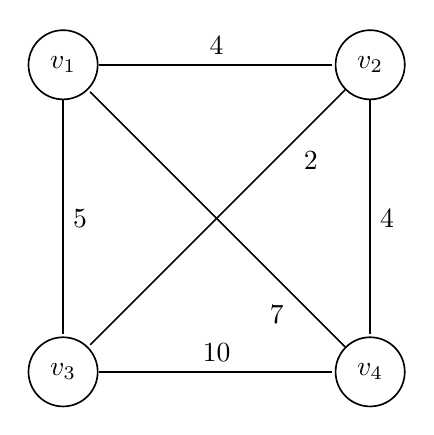
\begin{tikzpicture}[
    > = , % arrow head style
    shorten > = 1pt, % don't touch arrow head to node
    auto,
    node distance = 3cm, % distance between nodes
    semithick % line style
    ]

    \tikzset{every state}=[
    draw = black,
    thick,
    fill = white,
    minimum size = 1mm
    ]
    \node[state] (v1) {$v_1$};
    \node[state] (v2) [right=of v1] {$v_2$};
    \node[state] (v3) [below =of v1] {$v_3$};
    \node[state] (v4) [below =of v2] {$v_4$};
  
    \path[->] (v1) edge  node[]{4}(v2);
    \path[->] (v1) edge  node[]{5}(v3);
    \path[->] (v2) edge  node[pos=0.2,below right]{2} (v3);
    \path[->] (v3) edge  node[]{10}(v4);
    \path[->] (v2) edge  node[]{4}(v4);
    \path[->] (v4) edge  node[pos=0.2,below left]{7}(v1);
\end{tikzpicture}\\
 {\normalfont{Also according to definition \ref{subgraph}, the above graph is a subgraph of itself. Therefore it's weight can be calculated, where by definition \ref{weightofasubgraph}, the weight of}} G {\normalfont{is 32.}}\\
\\
According to Guichard \cite{guichard_2018}, trees are another useful class of graphs.
\begin{definition}
\label{tree}
A tree is a connected graph with no cycles. \normalfont{\cite{guichard_2018}}
\end{definition}
Having defined the basic graph theoretic concepts, it is now time to define harder concepts that use previous definitions. It is important to note that the following concepts can be applied to both weighted and unweighted graphs. Therefore, in the remaining definitions the graph being considered can either be weighted or unweighted.
\begin{definition}
\label{spanning subgraph}
H($V^\prime$,$E^\prime$) is a spanning subgraph of G(V,E) if H is a subgraph of G and $V^\prime$ = V. \normalfont{\cite{ray_2013}}
\end{definition}
There are many spanning subgraphs, however the ones that are relevant to this thesis are spanning trees and spanning cycles, the latter mostly known as Hamiltonian cycles.
\begin{definition}
A graph H is a spanning tree of G if H is a tree and H is a spanning subgraph of G. \normalfont{\cite{ray_2013}}
\label{spanning tree}
\end{definition}
\begin{definition}
\label{hamiltonian cycle}
Given a graph G, C is a Hamiltonian cycle in G if C is a cycle and C is a spanning subgraph of G. Also, a graph that contains a Hamiltonian cycle is called a Hamiltonian graph. \normalfont{\cite{ray_2013}}
\end{definition}
It is worth mentioning that definition \ref{hamiltonian cycle} holds because, cycles can be represented by Cycle graphs due to the construction discussed earlier. What follows now is an example that illustrates better definitions \ref{spanning subgraph}, \ref{spanning tree} and \ref{hamiltonian cycle}. 
\begin{example}
\label{example5}
{\normalfont{Let}} G {\normalfont{be the graph in example \ref{example4}. Then, according to definition \ref{spanning subgraph}, the two graphs below are two spanning subgraphs of}} G {\normalfont{because, they contain all the vertices of}} G {\normalfont{and are subgraphs of }}G .\\
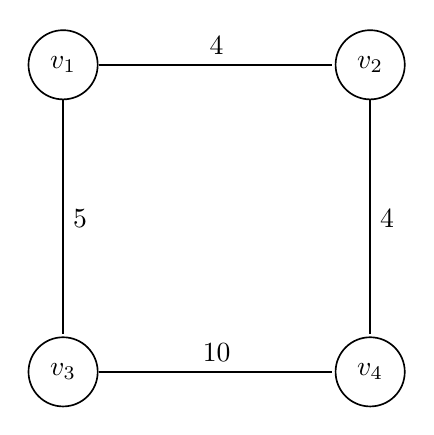
\begin{tikzpicture}[
    > = , % arrow head style
    shorten > = 1pt, % don't touch arrow head to node
    auto,
    node distance = 3cm, % distance between nodes
    semithick % line style
    ]

    \tikzset{every state}=[
    draw = black,
    thick,
    fill = white,
    minimum size = 1mm
    ]
    \node[state] (v1) {$v_1$};
    \node[state] (v2) [right=of v1] {$v_2$};
    \node[state] (v3) [below =of v1] {$v_3$};
    \node[state] (v4) [below =of v2] {$v_4$};
  
    \path[->] (v1) edge  node[]{4}(v2);
    \path[->] (v1) edge  node[]{5}(v3);
    \path[->] (v3) edge  node[]{10}(v4);
    \path[->] (v2) edge  node[]{4}(v4);
\end{tikzpicture}\\
\\
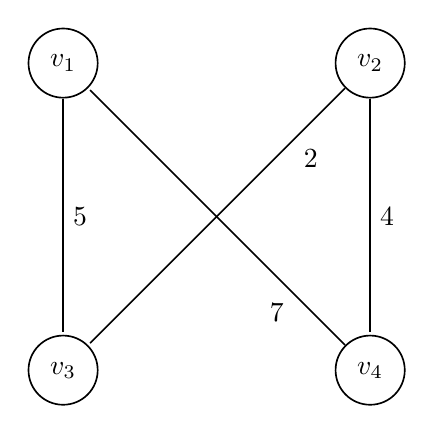
\begin{tikzpicture}[
    > = , % arrow head style
    shorten > = 1pt, % don't touch arrow head to node
    auto,
    node distance = 3cm, % distance between nodes
    semithick % line style
    ]

    \tikzset{every state}=[
    draw = black,
    thick,
    fill = white,
    minimum size = 1mm
    ]
    \node[state] (v1) {$v_1$};
    \node[state] (v2) [right=of v1] {$v_2$};
    \node[state] (v3) [below =of v1] {$v_3$};
    \node[state] (v4) [below =of v2] {$v_4$};
  
    \path[->] (v1) edge  node[]{5}(v3);
    \path[->] (v2) edge  node[pos=0.2,below right]{2} (v3);
    \path[->] (v2) edge  node[]{4}(v4);
    \path[->] (v4) edge  node[pos=0.2,below left]{7}(v1);
\end{tikzpicture}\\
{\normalfont{It must also be said that by definition \ref{hamiltonian cycle}, the above two graphs are Hamiltonian cycles in}} G {\normalfont{because, they are spanning subgraphs of}} G {\normalfont{and are Cycle sub-graphs of}} G. {\normalfont{Since the above graphs are subgraphs of }}G{\normalfont{, by definition \ref{weightofasubgraph}, their weight can be calculated by summing up the weights of the edges. Thus, the Hamiltonian cycles above have weight 23 and 18 respectively.}}\\
{\normalfont{Given the same graph }}G{\normalfont{ in example \ref{example4}, the two graphs below are spanning trees of }}G{\normalfont{ of weight 18 and 19 respectively.}}\\
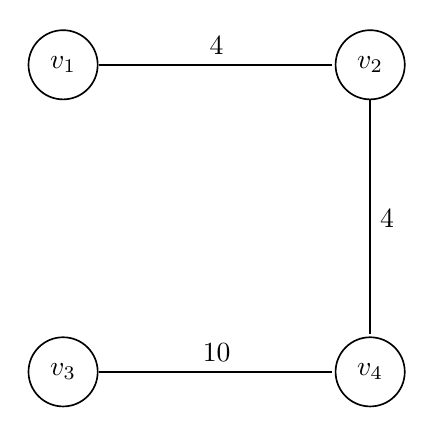
\begin{tikzpicture}[
    > = , % arrow head style
    shorten > = 1pt, % don't touch arrow head to node
    auto,
    node distance = 3cm, % distance between nodes
    semithick % line style
    ]

    \tikzset{every state}=[
    draw = black,
    thick,
    fill = white,
    minimum size = 1mm
    ]
    \node[state] (v1) {$v_1$};
    \node[state] (v2) [right=of v1] {$v_2$};
    \node[state] (v3) [below =of v1] {$v_3$};
    \node[state] (v4) [below =of v2] {$v_4$};
  
    \path[->] (v1) edge  node[]{4}(v2);
    \path[->] (v3) edge  node[]{10}(v4);
    \path[->] (v2) edge  node[]{4}(v4);
\end{tikzpicture}\\
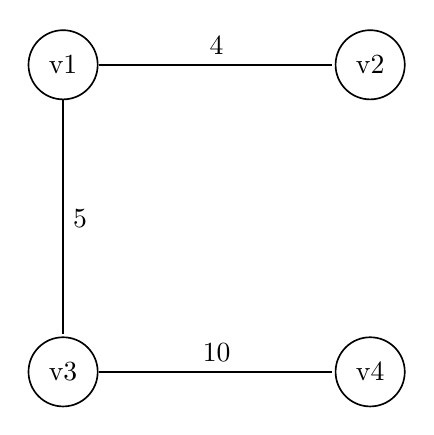
\begin{tikzpicture}[
    > = , % arrow head style
    shorten > = 1pt, % don't touch arrow head to node
    auto,
    node distance = 3cm, % distance between nodes
    semithick % line style
    ]

    \tikzset{every state}=[
    draw = black,
    thick,
    fill = white,
    minimum size = 1mm
    ]
    \node[state] (v1) {v1};
    \node[state] (v2) [right=of v1] {v2};
    \node[state] (v3) [below =of v1] {v3};
    \node[state] (v4) [below =of v2] {v4};
  
    \path[->] (v1) edge  node[]{4}(v2);
    \path[->] (v1) edge  node[]{5}(v3);
    \path[->] (v3) edge  node[]{10}(v4);
\end{tikzpicture}\\
{\normalfont{This example also shows that within the same weighted graph, there could be multiple Hamiltonian cycles and spanning trees of different weight.}}
\end{example}
Having defined Hamiltonian cycles and spanning trees, it is natural to ask whether there are necessary and sufficient conditions in a graph that guarantee it is Hamiltonian or that it contains a spanning tree as subgraph. In fact, theorem \ref{spanningtreetheorem} gives a necessary and sufficient condition for a graph to have a spanning tree.
\begin{theorem}
A graph G has a spanning tree $\iff$ it is connected {\normalfont{\cite{ray_2013}}}.
\label{spanningtreetheorem}
\end{theorem} 
\begin{proof}
($\implies$) Let $\mathit{G(V,E)}$ be a graph having a spanning tree $\mathit{T(V^\prime,E^\prime)}$ as one of it's subgraphs. Let $\mathit{v1, v2}$ $\in$ $\mathit{V}$. Since, $\mathit{T}$ is a spanning tree of $\mathit{G}$, then, $\mathit{T}$ is a spanning subgraph of $\mathit{G}$. Thus, $\mathit{v1, v2}$ $\in$ $V^\prime$. Also, since $\mathit{T}$ is a tree, $\mathit{T}$ must be connected. Therefore, $\exists$ a path $\mathit{P}$ joining vertices $\mathit{v_1}$ and $\mathit{v_2}$ in $\mathit{T}$. But since $\mathit{T}$ is a subgraph of G, then $\mathit{P}$ is also a path in $\mathit{G}$. Therefore $\mathit{G}$ must be connected.\\
($\Leftarrow$) Conversely, let $\mathit{G(V,E)}$ be a connected graph. Then, if $\mathit{G}$ has no cycles, $\mathit{G}$ itself must be a spanning tree. If $\mathit{G}$ has cycles, delete an edge from a cycle in $\mathit{G}$. Clearly, the resultant graph is still connected and contains one less cycle. Repeat this procedure untill no more cycles are left in the graph. Then, the resultant graph $\mathit{G^\prime}$ would be a connected subgraph of $\mathit{G}$ having no cycles(i.e a tree). Also, since by the deletion procedure, no vertex was deleted from $\mathit{G}$, $\mathit{G^\prime}$ is a spanning subgraph of $\mathit{G}$. Therefore $\mathit{G^\prime}$ is a spanning tree of $\mathit{G}$. \normalfont{\cite{ray_2013}}
\end{proof}
Theorem \ref{spanningtreetheorem} confirms that for a graph to have a spanning tree, the graph must be connected and vice-versa. Thus, for spanning trees, the necessary and sufficient condition is connectivity. However, the same cannot be said about Hamiltonian cycles because, no necessary and sufficient conditions are known for a graph to be Hamiltonian. In fact, there are sufficient conditions for a graph to be Hamiltonian, however, these conditions are not necessary. There are also necessary conditions, some of which are trivial, such as, if $\mathit{G}$ is Hamiltonian then G must be connected, but this is not necessary and sufficient. According to Guichard \cite{guichard_2018}, these sufficient conditions typically say that for a graph to be Hamiltonian it must have a lot of edges. But it is also argued in \cite{guichard_2018}, that these conditions are not necessary, because, there are Hamiltonian graphs that have few edges. For example, $\mathit{C_n}$ has only $\mathit{n}$ edges but is Hamiltonian. One such sufficient but not necessary condition for Hamiltonianicity is Ore's Theorem below.
\begin{theorem}[Ore's Theorem]
\label{ore's theorem}
Let G be a graph on n $\geq$ 3 vertices such that if v and w are not adjacent in G then deg(v) + deg(w) $\geq$ n. Then G is Hamiltonian. {\normalfont{\cite{ray_2013}}}
\end{theorem}
\begin{proof}
Suppose that $\mathit{G(V,E)}$ is a graph satisfying all the conditions in the theorem statement but is not Hamiltonian. Then since $\mathit{G}$ is not Hamiltonian and $K_n$ is Hamiltonian, $\mathit{G}$ must be a subgraph of $\mathit{K_n}$ having fewer edges than $\mathit{K_n}$. Therefore, add edges to $\mathit{G}$ between non adjacent vertices to obtain a subgraph $\mathit{H(V^\prime,E^\prime)}$ of $\mathit{K_n}$ such that adding an edge to $\mathit{H}$ would create a subgraph of $\mathit{K_n}$ which is Hamiltonian. Let $\mathit{u, v}$ $\in$ $V^\prime$ be 2 non-adjecent vertices in H. Since by construction $\mathit{G}$ is a subgraph of $\mathit{H}$, $\mathit{u, v}$ must be non-adjcent in $\mathit{G}$. Therefore $\mathit{deg(u) + deg(v) \geq n}$ in both G and H. Since adding an edge to $\mathit{H}$ creates a resultant graph that is Hamiltonian, then, adding an edge between $\mathit{u}$ and $\mathit{v}$ creates a Hamiltonian graph. Therefore, in $\mathit{H}$ there must be a path joining $\mathit{u}$ and $\mathit{v}$ containing all the vertices of $\mathit{H}$. Let the path be $\mathit{u = v_1, v_2, ..., v_n = v}$.\\
Now suppose $\mathit{deg(v_1)}$ = $\alpha$ in $\mathit{H}$. Now $\forall \mathit{i}, 1 <  i < \mathit{n}$, if there is an edge between $\mathit{u_1}$ and $\mathit{u_i}$ in $\mathit{H}$, then there must not be an edge between $\mathit{u_{i-1}}$ and $\mathit{u_n}$ because, $\mathit{u_1, u_i, u_{i+1}, ..., u_n, u_{i-1}, u_{i-2}, ..., u_1}$ would be a Hamiltonian cycle in $\mathit{H}$, thus H would be Hamiltonian. Therefore, $\mathit{deg(u_n)}$ $\leq$ $\mathit{n-1-\alpha}$\\
$\implies$ $\mathit{deg(u_1) + deg(u_n) \leq \alpha +  n-1 - \alpha}$ in $\mathit{H}$\\
$\implies$ $\mathit{deg(u_1) + deg(u_n) \leq n-1}$ in $\mathit{H}$\\
$\implies$ $\mathit{deg(u_1) + deg(u_n) < n}$ in $\mathit{G}$ since $\mathit{G}$ is a subgraph of $\mathit{H}$.\\
This contradicts the assumption that $\mathit{deg(u_1 = u) + deg(u_n = v) \geq n}$ in $\mathit{G}$ \\
Therefore, $\mathit{G}$ must be Hamiltonian. \cite{ray_2013}
\end{proof}
It is important to note that the above proof uses the fact that $K_n$ is Hamiltonian. This is true because any $C_n$ is always a subgraph of $K_n$. Therefore any $C_n$ that spans $K_n$ is a subgraph of $K_n$. Example \ref{example 6} below is a counter example to show why Ore's theorem gives a sufficient but not necessary condition.\\
\begin{example}
\label{example 6}
{\normalfont{Consider the graph}} $C_5$ below.
\\
\begin{tikzpicture}[
    > = , % arrow head style
    shorten > = 1pt, % don't touch arrow head to node
    auto,
    node distance = 3cm, % distance between nodes
    semithick % line style
    ]

    \tikzset{every state}=[
    draw = black,
    thick,
    fill = white,
    minimum size = 1mm
    ]
    \node[state] (v1) {$v_1$};
    \node[state] (v2) [below left =of v1] {$v_2$};
    \node[state] (v3) [below right =of v1] {$v_3$};
    \node[state] (v4) [below=of v2] {$v_4$};
    \node[state] (v5) [below=of v3] {$v_5$};

    \path[->] (v1) edge  node[]{}(v2);
    \path[->] (v2) edge  node[]{}(v4);
    \path[->] (v4) edge  node[]{}(v5);
    \path[->] (v5) edge  node[]{}(v3);
    \path[->] (v3) edge  node[]{}(v1);
\end{tikzpicture}\\
$C_5$ {\normalfont{above is Hamiltonian because it contains the Hamiltonian cycle}} $v_1, v_2, v_4, v_5, v_3, v_1$. {\normalfont{However,}} deg($v_1$) + deg($v_5$) = 4 $<$ 5 = n. {\normalfont{Therefore, the condition in Ore's Theorem is not a necessary condition}}.
\end{example} 
To conclude, these facts seem to indicate that determining whether a graph is Hamiltonian is a very difficult problem and that there are certain problems that are harder than other problems. In order to reason about such problems, some computational theory must first be established. This is done in the next subsection.
\subsection{Some Computational Theory}
After defining some important graph theoretic concepts, it is now time to present some important computational theory that will be used in later sections. The discussion will now proceed by defining two different types of problems and describing the relationship between them.
\begin{definition}
\label{optimization problems}
Suppose that a problem P has many possible solutions such that each solution has an associated value. Then P is an optimisation problem if P requires to find the solution with the best value.  \normalfont{\cite{cormen_leiserson_rivest_stein}}
\end{definition}
Therefore, according to definition \ref{optimization problems}, the aim of the algorithm solving an optimisation problem would then be to find the solution with the best (min/max) value. The solution with the best value is called an optimal solution to the problem, and it's value is known as the optimal value. An optimal solution is not termed as `the' optimal solution because, there could be many optimal solutions having the same optimal value. \cite{cormen_leiserson_rivest_stein} \\\\Another type of problems is called decision problems.
\begin{definition}
\label{decision problems}
Decision problems are problems whose solutions are either a yes or a no. \normalfont{\cite{cormen_leiserson_rivest_stein}}
\end{definition}
In \cite{cormen_leiserson_rivest_stein} it is argued that, given an optimisation problem, one can transform this optimisation problem into a decision problem such that, the decision problem is easier than the optimisation problem. Therefore, if some optimisation problem is easy to solve, the decision problem version is easy to solve as well \cite{cormen_leiserson_rivest_stein}. On the other hand, if the decision problem is hard to solve then this would mean that the original optimization problem is also hard to solve \cite{cormen_leiserson_rivest_stein}. Note that the notion of `hard' and `easy' problems will be defined rigorously later in this section. This concept was only mentioned here to show that there exists a relationship between optimisation problems and decision problems. Before going into harder computational theory, an example is given to undestand how an optimisation problem can be transformed into a related decision problem.
\begin{example}
\label{example decision/optimization}
{\normalfont{Two optimisation problems are:\\
1. The shortest path problem\\
2. The minimum weight spanning tree problem\\
Given a connected weighted graph}} G{\normalfont{, the shortest path problem is the task of finding a path}} P {\normalfont{between two vertices in}} G {\normalfont{such that, the weight of }}P {\normalfont{is the minimum amongst all paths joining these two vertices in }}G {\normalfont{\cite{hackerearth_blog}}}. {\normalfont{On the other hand, given a  connected weighted graph}} G {\normalfont{the minimum weight spanning tree problem is the task of finding a spanning tree in}} G {\normalfont{of minimum weight \cite{geeksforgeeks}. The shortest path problem is an optimsation problem because, from all the possible paths in the graph, a path having the optimal value (minimum weight) is chosen. In this case the best path is the path with minimum weight. Similarly, using the same reasoning, the minimum weight spanning tree problem is an optimisation problem. }}\\
{\normalfont{The decision problems related to these optimisation problems can be obtained by specifying a bound on the value to be optimized \cite{cormen_leiserson_rivest_stein}. Therefore, the decision problems related to the shortest path problem, and the minimum weight spanning tree problem defined in this example are:}}\\
{\normalfont{1.Given a connected weighted graph}} G, {\normalfont{two vertices}} u {\normalfont{and}} v, {\normalfont{and an integer}} k,{\normalfont{ does a path exist from}} u {\normalfont{to}} v {\normalfont{in}} G {\normalfont{of weight at most}} k?\\
{\normalfont{2.Given a connected weighted graph}} G, {\normalfont{and an integer}} k{\normalfont{, does}} G {\normalfont{contain a spanning tree of weight at most}} k?\\
{\normalfont{The above two problems are decision problems because the answer to these problems is either a yes or a no.}}
\end{example}
Reasoning about computational problems is usually done by analyzing the properties belonging to the algorithms that solve these problems. One property that is analyzed is called the running time of an algorithm. This is defined in definition \ref{running_time} below.
\begin{definition}
\label{running_time}
Given an input I, the running time of an algorithm A is the number of steps executed by A given I. The running time of an algorithm A can be represented by the function T $:$ $\mathbb{N}$ $\mapsto$ $\mathbb{N}$ were the domain represents the size of the input, and the co-domain represents the amount of steps taken by the algorithm to execute given an input size. {\normalfont{\cite{cormen_leiserson_rivest_stein}, \cite{adamchik_2009}}}
\end{definition}
The following is an example on how the running time of an algorithm can be constructed.
\begin{example}
\label{example_running}
{\normalfont{Consider an algorithm that performs the addition of two}} n-{{\normalfont{bit strings. Then if the addition of 2 bits takes}}} a {\normalfont{computational steps, the addition of 2}} $\mathit{n-}${\normalfont{bit strings will take}} a $\times$ n {\normalfont{steps, since, each computation must be performed}} n {\normalfont{times (i.e on each bit in the string). Therefore, the running time of this algorithm for an input of size}} n {\normalfont{can be represented by the function,\\}} T(n) = a $\times$ n. {\normalfont{\cite{cormen_leiserson_rivest_stein}, \cite{adamchik_2009}}}
\end{example}
Expressing the running time in this way seems pretty easy to understand. However, it has problems. Typically, the running time of an algorithm is fixed for any input, however, the running time function is not defined on the actual inputs, but, on the input sizes. As a result, since the same input size might represent different inputs, there could be different running times for the same input size $\mathit{n}$, as this depends on which input is given. This means that for any input size $\mathit{n}$, there are different running time functions giving different running times. These different running time functions represent the different cases that could arise in an algorithm given any input size $\mathit{n}$. The most important runnning time functions are the worst-case running time, the best-case running time and the average-case running time. The worst/best/average case running time are the longest/shortest/average running time of an algorithm given any input of size $\mathit{n}$ respectively. Therefore the problem is what running time function should be used to reason about algorithms. Although the average-case running time generally has a greater practical significance, it is often very difficult to compute. Therefore, the worst-case running time is usually used, that is, finding the running time function that gives the worst-case running time for any input of size $\mathit{n}$. The worst-case running time of an algorithm is an upper bound to all other running times, therefore, this assures that the algorithm will never get a longer running time for any input of size $\mathit{n}$. So, if the worst case running time is polynomial in the input size, then we know that the problem is in class P (These terms will be defined below).  \cite{cormen_leiserson_rivest_stein}, \cite{adamchik_2009}\\\\
Another problem is that, the running time of an algorithm can be difficult to compute precisely because it depends on the computer the algorithm is executed on. This informally means that, an algorithm may need different amount of computational steps on different computers for the same input. For example, the number of steps taken for adding 2-bits as seen in example \ref{example_running}, may be different on different computers, resulting into running time functions that represent the same worst/best/average running time case, differing only in multiplicative constants and low order terms. To get around this problem, a mechanism that identifies a common property between all running time functions is needed. This mechanism is called asymptotic analysis. This means making the input size increase without bound so that only the order of growth of the running time function is relevant. This works because, as the input size increases, the low-order terms and multiplicative constants of the running time function get dominated by the size of the input itself. This means that, given any running time function, the low-order terms and multiplicative constants of the function can be ignored leaving only the order of growth (which is common across all running time functions representing the same best/worst/average running time case). In a running time function, the order of growth is given by the highest order term. This is because, the highest order term has the greatest effect on the running time function as the input size increases. For example, given the running time function $\mathit{T(n) = an^2+bn+c}$, $\mathit{n^2}$ is the term that increases the running time the most as the input size increases without bound. \cite{cormen_leiserson_rivest_stein}, \cite{adamchik_2009} \\\\
The following example is used to explain better what has been discussed in the previous paragraph.
\begin{example}
{\normalfont{Suppose that the }} n-{\normalfont{bit addition algorithm in example \ref{example_running}, has a worst-case running time function}} T(n) = a $\times$ n {\normalfont{on computer}} A {\normalfont{and a worst-case running time function}} T(n) = b $\times$ n {\normalfont{on computer}} B {\normalfont{where,}} a/b {\normalfont{represent the number of computational steps required to perform 2-bit addition on computers}} A/B {\normalfont{respectively. The asymptotic analysis of the algorithm concludes that, the}} n-{\normalfont{bit addition algorithm has an }} $n^2$ {\normalfont{ asymptotic behaviour. Note that this is common to both running time functions}}. {\normalfont{\cite{cormen_leiserson_rivest_stein}, \cite{adamchik_2009}}}
\end{example}
To express the asymptotic behaviour of functions mathematically, asymptotic notations are normally used. One of these notations is called the Big O Notation, whose exact definition is given below.
\begin{definition}
\label{bigonotation}
Let f $:$ $\mathbb{N}$ $\mapsto$ $\mathbb{N}$ and g $:$ $\mathbb{N}$ $\mapsto$ $\mathbb{N}$ be two monotonic functions. Then f(n) = O(g(n)) if $\exists$ c $>$ 0 and $n_0$ $>$ 0 such that f(n) $\leq$ cg(n) $\forall$ n $\geq$ $n_0$. \normalfont{\cite{adamchik_2009}} 
\end{definition}
Definition \ref{bigonotation} implicitly states that when writing $\mathit{f(n) = O(g(n)), g(n)}$ is an upperbound to $\mathit{f(n)}$ as the input size $\mathit{n}$ grows without bound \cite{adamchik_2009}. Therefore, if $\mathit{f(n)}$ is the worst case running time function of an algorithm and $\mathit{f(n) = O(g(n))}$, then it is guaranteed that as $\mathit{n \rightarrow \infty}$ the algorithm will never get a running time longer than $\mathit{g(n)}$ times some constant. Note that definition \ref{bigonotation} can be used even for the asymptotic analysis of the average and best case running times. However, unless otherwise stated, it can be assumed that in this thesis Big O Notation will be used for the worst-case asymptotic analysis of algorithms. The following is a continuation to example \ref{running_time}.
\begin{example}
\label{bigonotationexample}
{\normalfont{By example \ref{running_time}, the algorithm that performs two}} n-{\normalfont{bit addition has a running time function}} T(n)= an. {\normalfont{Therefore, by definition \ref{bigonotation},}} T(n) = O(n) {\normalfont{because, since}} a  {\normalfont{is a natural number}} $\exists$ z $\geq$ a {\normalfont{such that,}} an $\leq$ zn $\forall$ n $\in$ $\mathbb{N}$. {\normalfont{Therefore at each step, the order of growth of}} T(n) {\normalfont{is linear with respect to the input size}} n.
\end{example}
It is important to note that if $\mathit{T(n) = O(g(n))}$, then, $\mathit{T(n) = O(h(n))}$ if $\mathit{h(n)}$ has a higher order of growth than $\mathit{g(n)}$. For example, in example \ref{bigonotation} $\mathit{T(n) = O(n^2)}$ as well since, $\mathit{n^2}$ is an upperbound to $\mathit{n}$ therefore, it is an upperbound to $\mathit{T(n)}$. However, unless otherwise stated, it can be assumed that whenever $\mathit{T(n) = O(g(n))}$, $\mathit{g(n)}$ is a tight asymptotic bound to $\mathit{T(n)}$. A tight asymptotic bound to $\mathit{T(n)}$ is a function $\mathit{g(n)}$ such that, if $\mathit{T(n)=O(f(n))}$ then $\mathit{g(n)=O(f(n))}$.\\\\
So we have the following definition.
\begin{definition}
\label{time_complexity}
Given a function g(n) and an algorithm A having a running time function T(n), A is said to have a time complexity of O(g(n)) if T(n) = O(g(n)). \normalfont{\cite{adamchik_2009}} 
\end{definition}
Definition \ref{time_complexity} does not apply only to the worst case running time function. However, recall that when discussing running time functions it was said that it can be assumed that, the worst-case running time function is taken. Therefore, it can be assumed that the worst-case running time function is taken when saying that an algorithm has an $\mathit{O(g(n))}$ time complexity, or when saying that an algorithm is an $\mathit{O(g(n))}$ algorithm. This will sometimes also be termed as, the worst-case time complexity of the algorithm. Note that when it is said that a problem can be solved in $\mathit{O(g(n))}$ time, this means the problem can be solved by an algorithm that has an $\mathit{O(g(n))}$ worst-case time complexity.\\\\
The following table summarizes some of the most common time complexities encountered in computational theory, and what they are commonly known as. The table was adapted using information from \cite{big_o_notation_explained} and \cite{carter_1999}.
\begin{table}[!htbp]
  \begin{center}
    \caption{Time Complexities and Terminology Used.}
    \label{tab:table1}
    \begin{tabular}{l|c} % <-- Alignments: 1st column left, 2nd middle and 3rd right, with vertical lines in between
      \textbf{Time Complexity} & \textbf{Terminology Used}\\
      \hline
      O(1)                          & Constant time    \\
     $O(\mathit{\log n})$          & Logarithmic time \\
     $O(\mathit{n})$               & Linear time      \\
     $O(\mathit{n \log n})$        & Log-linear time  \\
     $O(\mathit{n^2})$             & Quadratic time   \\
     $O(\mathit{n^c})$, $\mathit{c > 0}$ constant & Polynomial time  \\
     $O(\mathit{a^n})$, $\mathit{a \geq 2}$ constant & Exponential time \\
     $O(\mathit{n!})$              & Factorial time
    \end{tabular}
  \end{center}
\end{table}
\\In Table \ref{tab:table1}, the time-complexities are ordered in ascending order of growth \cite{big_o_notation_explained}. This means that, for example, constant time algorithms have a smaller order of growth than logarithmic time algorithms. It must be noted that the higher the order or growth, the more steps the algorithm needs to execute for any input and therefore, the less efficient it is. In general, problems that can be solved in polynomial time are tractable problems \cite{cormen_leiserson_rivest_stein}. On the other hand, problems that require superpolynomial (exponential/factorial) time algorithms to be solved are intractable problems \cite{cormen_leiserson_rivest_stein}. In general, tractable problems are considered to be easy to solve, whereas intractable problems are hard to solve. Table \ref{tab:table2} below is constructed to show why problems that can be solved in polynomial time are tractable, whilst, problems that cannot be solved in polynomial time are intractable. Table \ref{tab:table2} gives the execution time of any algorithm given an input of size $\mathit{10}$, $\mathit{100}$ or $\mathit{1000}$, provided that the algorithm's time complexity is $\mathit{O(n)}$, $\mathit{O(n^2)}$, $\mathit{O(2^n)}$ or $\mathit{O(n!)}$.
\begin{table}[!htbp]
  \begin{center}
    \caption{Execution Time Given Input Size and Time Complexity}
    \label{tab:table2}
    \begin{tabular}{l|c|c} % <-- Alignments: 1st column left, 2nd middle and 3rd right, with vertical lines in between
      \textbf{\backslashbox{Time Complexity}{Input Size}} & \textbf{10} & \textbf{100}\\
      \hline
     $\mathit{O(n)}$ & $\mathit{1{\times10^{-8} seconds}}$ & $\mathit{1{\times10^{-7} seconds}}$\\
     $\mathit{O(n^2)}$ & $\mathit{1{\times10^{-7} seconds}}$ & $\mathit{1{\times10^{-5} seconds}}$     \\
     $\mathit{O(2^n)}$ & $\mathit{1.024{\times10^{-6} seconds}}$ & $\mathit{1.2676{\times10^{21} seconds}}$\\
     $\mathit{O(n!)}$ & $\mathit{3.6288{\times10^{-3} seconds}}$ & Very large to compute
    \end{tabular}
  \end{center}
\end{table}
\begin{table}[!htbp]
    \begin{tabular}{l} % <-- Alignments: 1st column left, 2nd middle and 3rd right, with vertical lines in between
      \textbf{1000}\\
      \hline
     $\mathit{1{\times10^{-6} seconds}}$\\
     $\mathit{1{\times10^{-3} seconds}}$     \\
     Very large to compute  \\
     Very large to compute
    \end{tabular}
\end{table}
\\\\Table \ref{tab:table2} above was adapted from \cite{pettis}. In Table \ref{tab:table2} above it is assumed that the machine the algorithms can be executed on perform $\mathit{10^9}$ computational steps per second \cite{pettis}. It can be concluded from Table \ref{tab:table2} above that, as the size of the input increases, only the polynomial functions have small values. This means that a polynomial time algorithm does not have a very large execution time even if the size of the input is increased substantially. On the other hand, an algorithm with an exponential or factorial time complexity has a very large execution time, because, the rate of growth of the time complexity function is very large.
\\\\The following is an example to wrap-up all the time complexity concepts discussed so far.
\begin{example}
\label{time_complexity_example}
{\normalfont{In example \ref{bigonotationexample},}} T(n) = O(n). {\normalfont{Therefore according to definition \ref{time_complexity}, the}} n-{\normalfont{bit addition algorithm has a time complexity of}} O(n). {\normalfont{Therefore by Table \ref{tab:table1}, the}} n-{\normalfont{addition algorithm has a linear time complexity, or simply is a linear-time algorithm. As a result, the}} n-{\normalfont{bit addition problem can be solved in linear time}}.
\end{example}
In what has been presented so far in this section it has always been assumed that, any problem has an algorithm that solves it. However, this is not the case because there are computational problems that cannot be solved by any computer, no matter how much processing power and time is dedicated to them. In addition to that, there are problems that can be solved in polynomial time and others which cannot. This seems to indicate that there are several classes of problems. One of these classes is the class P defined below. \cite{cormen_leiserson_rivest_stein}
\begin{definition}
\label{P}
The class P consists of all the problems that can can be solved in polynomial time. {\normalfont{\cite{cormen_leiserson_rivest_stein}}}
\end{definition}
Therefore according to Definition \ref{P}, the class P consists of tractable problems. An example of a problem in the class $\mathit{P}$ is the $\mathit{n}$-bit addition problem defined in Example \ref{example_running}. The $\mathit{n}$-bit addition problem is in the class P because, it can be solved in linear time (as discussed in example \ref{time_complexity_example}). Apart from the class P, there is also the class NP. The following definition helps in defining the class NP.
\begin{definition}
\label{polynomial_time_verification}
A problem can be verified in polynomial time if given a solution to the problem, the solution can be checked by an algorithm if it is correct or not in polynomial time. {\normalfont{\cite{cormen_leiserson_rivest_stein}}}
\end{definition}
The following example explains the concept of polynomial time verification.
\begin{example}
\label{example_polynomial_time_verification}
{\normalfont{To explain polynomial time verification, the Hamiltonian Cycle problem is going to be used. Given a graph}} G(V,E){\normalfont{, the Hamiltonian cycle problem is the task of determing whether}} G {\normalfont{has a Hamiltonian cycle \cite{cormen_leiserson_rivest_stein}. A solution to the Hamiltonian cycle problem is a cycle}} S = $v_1$, ..., $v_n$ {\normalfont{of }}$|$V$|$ = n {\normalfont{vertices. Therefore, to confirm that the Hamiltonian cycle problem is verifiable in polynomial time, }}S {\normalfont{must be checked if it is a Hamiltonian cycle or not in polynomial time. This can be done by creating an algorithm that checks if }} $\forall$ i $\in$ [n-1], \{$v_i, v_{i+1}\} \in$ E and \{$v_n$, $v_1\} \in$ E. {\normalfont{Therefore, the checker algorithm has a worst case}} O(n) {\normalfont{time complexity because, it must check all edges in the cycle. Hence, the checker algorithm takes polynomial time to execute. As a result, the Hamiltonian cycle problem can be verified in polynomial time.}}
\end{example}
Now the class NP can be defined.
\begin{definition}
\label{NP}
The class NP consists of all decision problems that can be verified in polynomial time. {\normalfont{\cite{cormen_leiserson_rivest_stein}, \cite{geeksforgeeks_2018_2}}}
\end{definition}
 It is important to note that according to definition \ref{NP}, a problem $\mathit{A}$ is in the class NP if $\mathit{A}$ is a decision problem. This will not be a limiting factor because, as discussed before, every optimization problem can be transformed into a related decision problem by specifying a bound on the solution to be optimized (see example \ref{example decision/optimization}). Reasoning about decision problems is easier because, the related decision problem is not harder than the original optimisation problem. As a result, one can prove that an optimisation problem cannot be solved in polynomial time by showing that, the related decision problem cannot be solved in polynomial time.\cite{cormen_leiserson_rivest_stein}\\\\
Another important class of problems is the class of NP-Complete problems. To define this class, a reduction algorithm must first be defined.
\begin{definition}
\label{reduction_algorithm}
Suppose that A and B are two decision problems. A reduction algorithm is an algorithm that transforms any instance (input) $\alpha$ of A into an instance $\beta$ of B with the following properties:
\begin{itemize}
   \item The algorithm takes polynomial time to execute
   \item The solution to $\alpha$ is yes $\iff$ the solution to $\beta$ is yes. {\normalfont{\cite{cormen_leiserson_rivest_stein}}}
\end{itemize} 
\end{definition}
A reduction algorithm has important applications in computational theory. In fact, suppose that there are two decision problems $\mathit{A}$ and $\mathit{B}$ such that an instance $\mathit{\alpha}$ of the problem $\mathit{A}$ needs to be solved in polynomial time. Suppose also that, $\mathit{B}$ can be solved in polynomial time using algorithm $\mathit{B^\star}$ and there exists a reduction algorithm $\mathit{R}$ from $\mathit{A}$ to $\mathit{B}$. Then $\mathit{A}$ can be solved in polynomial time in the following way :
 \begin{itemize}
	\item Use $\mathit{R}$ to transform $\mathit{\alpha}$ into an instance $\mathit{\beta}$ of $\mathit{B}$
	\item Execute $\mathit{B^\star}$ on the input $\beta$ to get answer $\gamma$ = yes/no
	\item Give $\mathit{\gamma}$ as an answer for $\mathit{\alpha}$.
\end{itemize} 
It is important to note that $\mathit{A}$ can be solved in polynomial time because, the total time of the above procedure is polynomial. The above procedure is polynomial because, the total time of executing two polynomial time algorithms is the summation of two polynomials, which by properties of polynomials is still polynomial. It is important to note that, the above could only be done because the solution to $\alpha$ is yes $\iff$ the solution to $\beta$ is yes. \cite{cormen_leiserson_rivest_stein}\\\\
Another important application of reduction algorithms is to show that a polynomial time algorithm does not exist for a particular decision problem. Let $\mathit{A}$ and $\mathit{B}$ be decision problems such that $\mathit{A}$ cannot be solved in polynomial time. Suppose that $\exists$ a reduction algorithm $\mathit{P}$ from $\mathit{A}$ to $\mathit{B}$. Then it can be shown that $\mathit{B}$ cannot be solved in polynomial time because, if $\mathit{B}$ can be solved in polynomial time, then $\mathit{P}$ can be used to transform any instance $\alpha$ of $\mathit{A}$ into an instance $\beta$ of $\mathit{B}$ were again, $\alpha$ can be solved in polynomial time as discussed in the previous paragraph. Since $\alpha$ is arbitrary, $\mathit{A}$ can be solved for all inputs in polynomial time and hence, $\mathit{A}$ can be solved in polynomial time. This contradicts the assumption that $\mathit{A}$ cannot be solved in polynomial time. Therefore, when using a reduction algorithm from a decision problem $\mathit{A}$ to a decision problem $\mathit{B}$, one implicitly makes the statement that decision problem $\mathit{B}$ is as hard (in terms of tractability as discussed before) as decision problem $\mathit{A}$. If not, this would contradict properties that belong to the problem $\mathit{A}$. \cite{cormen_leiserson_rivest_stein}\\\\
After defining reduction algorithms, the class of NP-Complete problems can now be defined.
\begin{definition}
\label{NPC}
A decision problem A is in the class NP-Complete (NPC) if A is in NP and A is as hard as any problem in NP. {\normalfont{\cite{cormen_leiserson_rivest_stein}} }
\end{definition}
In other words, definition \ref{NPC} states that for a problem $\mathit{A}$ to be in NPC, $\mathit{A}$ must be in NP and that any problem in NP can be transformed using a reduction algorithm into $\mathit{A}$. Therefore, to show that a problem $\mathit{A}$ is in NPC, one must show that it is in NP, and that every problem in NP can be reduced to $\mathit{A}$. Showing that $\mathit{A}$ is in NP is not difficult because, it only requires to show that an arbitrary solution of $\mathit{A}$ can be verified in polynomial time. On the other hand, showing that every problem in NP is reducible to $\mathit{A}$ may seem diffcult because, this requires checking that every problem in NP can be reduced to $\mathit{A}$ \cite{geeksforgeeks_2018_2}. However, this is not the case because reduction algorithms are transitive \cite{geeksforgeeks_2018_2}. Hence, considering a known NP-Complete problem $\mathit{H}$, since $\mathit{H}$ is NP-Complete, every problem in NP can be reduced to $\mathit{H}$. Therefore, if one can find a reduction algorithm from $\mathit{H}$ to $\mathit{A}$, then by transitivity of reduction algorithms, every problem in NP can be reduced to $\mathit{A}$ using a reduciton algorithm \cite{geeksforgeeks_2018_2}.\\\\
The classes P, NP and NPC have very important implications in computational theory. One of the most important problems in computational theory is whether P = NP. It is known that P $\subseteq$ NP. This is true because, since every problem in P can be solved in polynomial time, then implicitly the polynomial time verification has been done by the algorithm solving the problem. Therefore, every problem in P is in NP and hence, P $\subseteq$ NP. Showing that NP $\subseteq$ P may seem to be easy as well. In fact, to show that NP $\subseteq$ P, one only needs to show that $\exists$ an NP-Complete problem $\mathit{C}$ that can be solved in polynomial time, because, by the NP-Completness of $\mathit{C}$, every problem in NP can be reduced using a reduction algorithm to $\mathit{C}$ and hence, every problem in NP could be solved in polynomial time since the reduction algorithm and the algorithm solving $\mathit{C}$, would take a total time that is still polynomial. However, no polynomial time algorithm has yet been discovered for any problem in NPC. In addition to this, no one has yet been able to prove that such polynomial time algorithms do not exist for NP-Complete problems. This essentially means that, the NP $\subseteq$ P problem is still an open question. \cite{cormen_leiserson_rivest_stein}\\\\
After defining the important computational theory, it is now time to define the Travelling Salesman Problem, and present important properties about it. This will all lead to showing that the Travelling Salesman Problem is NP-Complete, hence, showing that no polynomial time algorithm has yet been discovered to solve the Travelling Salesman Problem. All of this will be done in the next section.
\newpage
\section{The Travelling Salesman Problem}
After defining all the graph theoretic concepts and computational theory required, it is now time to define the Travelling Salesman Problem. The Travelling Salesman Problem is defined in definition \ref{TSP} below.
\begin{definition}
\label{TSP}
Given a complete weighted graph G, the Travelling Salesman Problem (TSP) is the problem of finding a minimum weight Hamiltonian cycle in G. {\normalfont{\cite{bondy_murty_1982}}}
\end{definition}
According to definition \ref{TSP}, for the TSP to be defined on a weighted graph $\mathit{G}$, $\mathit{G}$ must be complete. However, this is not a limiting factor because, every weighted graph $\mathit{G^\prime}$ can be converted into a complete weighted graph, by adding the missing edges in $\mathit{G^\prime}$ with a very large weight. As a result, if $\mathit{G^\prime}$ is an incomplete weighted Hamiltonian graph, the minimum weight Hamiltonian cycle in $\mathit{G^\prime}$ would never be effected when transforming $\mathit{G^\prime}$ into a complete graph, because, since the missing edges have a very large weight, they can never be part of the minimum weight Hamiltonian cyle when added. Note that if $\mathit{G^\prime}$ is not Hamiltonian, the minimum weight Hamiltonian cycle after transforming $\mathit{G^\prime}$ into a complete graph would be very large. Therefore, since there is no loss of generality, it can be assumed that complete graphs are always being considered when discussing the TSP.\\\\
Definition \ref{TSP} also specifies indirectly that, if $\mathit{G}$ is a complete weighted graph then $\mathit{G}$ is Hamiltonian, otherwise, if not, no Hamiltonian cycle can be found. This is true because, considering the complete graph $\mathit{K_n}$ on $\mathit{ n \geq 3}$ vertices, every Hamiltonian cycle consisting of $\mathit{n}$ vertices is in $\mathit{K_n}$. This property holds because, any two disinct vertices in $\mathit{K_n}$ are adjacent. Note that for the TSP, $K_2$ and $K_1$ are implicitly excluded because, by definition \ref{cycle}, cycles are defined on graphs having at least 3 vertices.\\ 
\\
The following example is used to clearly explain what the TSP defined in definition \ref{TSP} is all about.
\begin{example}
\label{example_2.1}
{\normalfont{Consider the complete graph}} $K_4$ {\normalfont{with the weight function}} f {\normalfont{defined in example \ref{example4}. The distinct Hamiltonian cycles (Hamiltonian cycles that differ in at least one edge of}} G{\normalfont{) in }}G {\normalfont{are:}}
\begin{itemize}
   \item $v_1$, $v_2$, $v_3$, $v_4$, $v_1$ {\normalfont{with weight}} 23
   \item $v_1$, $v_3$, $v_4$, $v_2$, $v_1$ {\normalfont{with weight}} 23
   \item $v_1$, $v_3$, $v_2$, $v_4$, $v_1$ {\normalfont{with weight}} 18
\end{itemize} 
{\normalfont{Therefore, by definition \ref{TSP}, the solution to the TSP on the instance}} G {\normalfont{would be the minimum weight Hamiltonian cycle}} $v_1$, $v_3$, $v_2$, $v_4$, $v_1$. {\normalfont{Note that}} $K_4$ {{\normalfont{has}}} 3 {\normalfont{distinct Hamiltonian cycles. This fact is a special case of lemma \ref{lemma_disinct_hamiltonian_cycles} for any}} $K_n$.
\end{example}
Example \ref{example_2.1} may show that, to solve the TSP on a graph instance, one can do it by a brute-force algorithm. A brute-force algorithm for TSP is one that computes all the Hamiltonian cycles in a graph and chooses the one of least weight as a soltution \cite{Sanchit}. However, according to Krivelevich \cite{Krivelevich}, $\mathit{K_n}$ contains $\mathit{\frac{(n-1)!}{2}}$ distinct Hamiltonian cycles. Therefore, a brute-force algorithm is inefficient because it must generate all the distinct Hamiltonian cycles in the graph taking factorial time to do so \cite{Sanchit}. This means that the brute-force algorithm is a factorial time algorithm.
\\\\Lemma \ref{distinct_hamiltonian_cycles} below confirms that, the complete graph $\mathit{K_n}$ on $\mathit{n\geq 3}$ vertices contains $\mathit{\frac{(n-1)!}{2}}$ distinct Hamiltonian cycles. Therefore, it confirms that a brute-force algorithm cannot efficiently solve the TSP.
\begin{lemma}
\label{distinct_hamiltonian_cycles}
For n $\geq$ 3, the complete graph on n vertices has $\frac{(n-1)!}{2}$ distinct Hamiltonian cycles \cite{mathematics_stack_exchange_2012}.
\end{lemma}
\begin{proof}
Let $K_n$ be the complete graph on $n \geq 3$ vertices. Since $\forall$ $u$,$v$ $\in$ $V(K_n)$, $u$ $\ne$ $v$ $\implies$ $\{u,v\}$ $\in$ $E(K_n)$, then, every permutation of $V(K_n)$ must represent a path in $K_n$ containing every vertex of $K_n$ and vice-versa (1-1 correspondence). Let $A$ be the set of all permutations of $V(K_n)$, and $B$ be the set of all paths in $K_n$ containing every vertex of $K_n$. Now, let $H$ be the set of all Hamiltonian cycles (not necessarily distinct) in $K_n$. Now, each Hamiltonian cycle can be transformed into a Hamiltonian path by removing the last vertex of the cycle. On the other hand, each Hamiltonian path can be transformed into a Hamiltonian cycle by repeating the first vertex as the last vertex. Therefore, there is a 1-1 correspondence between $H$ and $B$. As a result by the transitivity of 1-1 correspondence, there is a 1-1 correspondence between $A$ and $H$. Hence, the number of Hamiltonian cycles in $K_n$ is equal to the number of permutations of $V(K_n)$. However, different permutations of $V(K_n)$ may represent the same Hamiltonian Cycle in $K_n$ since, the same edges would be used from $E(K_n)$ but in a different order of the vertices. In fact, consider the Hamiltonian Cycle $C$ represented by the permutation $v_1$, $v_2$, ..., $v_n$. In terms of Hamiltonian cycles, the permutation $v_1$, $v_2$, ...$v_n$ is the same as the permutation $v_2$, ..., $v_n$, $v_1$ because, the same edges in $E(K_n)$ are used. Therefore, for each Hamiltonian cycle in $K_n$, we can have $n$ permutations representing the same cycle each starting from a different vertex, but using the same edges. Also, for each of these $n$ permutation representations, the reverse of each of these permutations represent the same Hamiltonian Cycle, with the difference being that the cycle is traversed in reverse order, thus we have $2n$ permutations representing the same Hamiltonian Cycle. Therefore, the number of distinct permutations is $\frac{n!}{2n}$ = $\frac{(n-1)!}{2}$.
\end{proof}
Note that the proof for Lemma \ref{distinct_hamiltonian_cycles} was constructed from ideas in \cite{mathematics_stack_exchange_2012}.\\\\
As discussed in previous paragraphs, Lemma \ref{distinct_hamiltonian_cycles} confirms that a brute-force algorithm will not be efficient enough to solve the TSP for large instance sizes. This means that, we can either try and design a new algorithm that solves the TSP in polynomial time, or, try and prove that TSP is an NP-Complete problem. The latter would confirm that no polynomial time algorithm is known for the TSP. However, at the same time this does not exclude that a polynomial time algorithm that solves TSP does not exist.
\subsection{Heuristics}
\subsection{The Ant Colony Algorithm}
\newpage
\section{Experimental Data}
\newpage
\section{Conclusion}
\newpage
\bibliography{bibliography}
\bibliographystyle{IEEEtran}
\end{document}